\documentclass[10pt]{article}
\setlength{\topmargin}{-0.5in}
\setlength{\textwidth}{6.5in}
\setlength{\oddsidemargin}{0in}
\setlength{\textheight}{9in}
\newcommand{\vecx}{\mathbf{x}}

%\usepackage{multirow}
%\usepackage{rotating}
\usepackage[fleqn]{amsmath}
\usepackage{nicefrac}

\usepackage{amsfonts}
\usepackage{natbib}
\usepackage{palatino}
\usepackage{url}
\usepackage{graphicx}

\newcommand{\wlin}{\mathbf{w}_{\text{lin}}}

\begin{document}

\title{CSE 417T: Homework 5 Solution Sketch}

\maketitle

\noindent \textbf{Note:} These are not intended to be comprehensive,
just to help you see what the answers should be.


\begin{enumerate}

\item

Below are two figures to demonstrate the ``shape'' of the curves. The idea is that both the train error and test error keep decreasing when the number of weak hypotheses increase.  No overfitting is observed.

\begin{figure}[h]
\begin{center}
    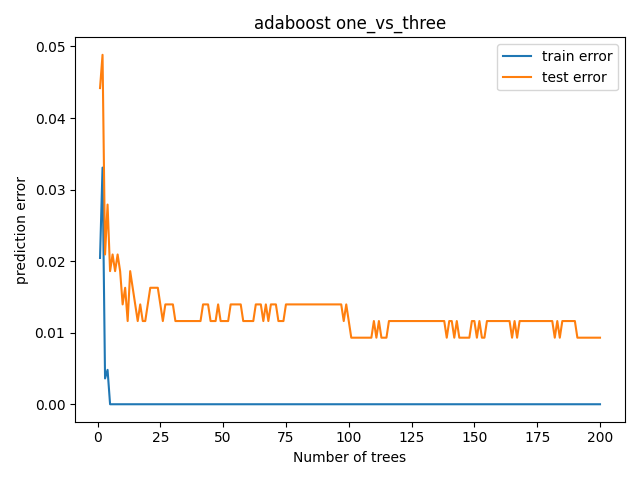
\includegraphics[width=.45\textwidth]{1vs3.png}
    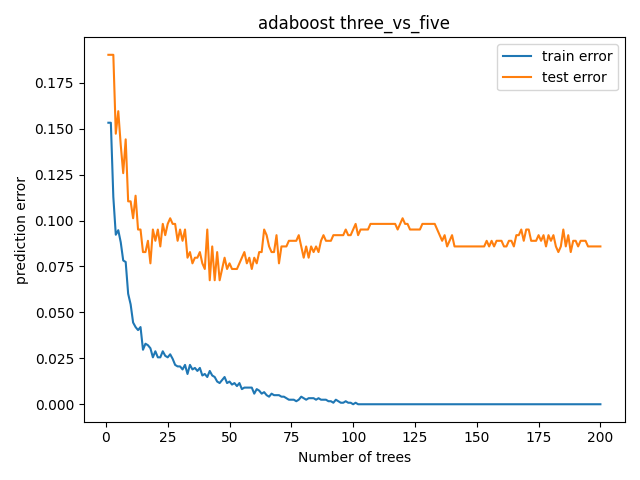
\includegraphics[width=.45\textwidth]{3vs5.png}
\end{center}
\end{figure}

\item
  The three closest points are $(3,
  5), (3, 8), (2, 11)$. For the 3-NN average, we would predict the
  average $y$ values of these three points, which would give us 8. 


\item The mapping is easy to compute. 
\begin{itemize}
	\item $[-1, -1]$ maps to $[-1, +1]$; 
  	\item $[-1, +1]$ maps to $[-1, -1]$; 
    \item $[+1, -1]$ maps to $[+1, -1]$; 
    \item $[+1, +1]$ maps to $[+1, +1]$. 
\end{itemize}

The maximal margin separator in the new space is the line $x_1 x_2 = 0$, with a margin of 1. 
In the original space, this is equivalent to $x_1 = 0$ and $x_2 = 0$, which you can think of as the limit of a hyperbolic separator with two branches.

\item The squared Euclidean distance is the dot product of $\Phi(\vecx_i)
  - \Phi(\vecx_j)$ with itself. This can be written as $\Phi(\vecx_i)
  \cdot \Phi(\vecx_i ) + \Phi(\vecx_j) \cdot \Phi(\vecx_j) - 2
  \Phi(\vecx_i) \cdot \Phi(\vecx_j)$, which is just $K(\vecx_i,
  \vecx_i) + K(\vecx_j, \vecx_j) - 2 K (\vecx_i, \vecx_j)$.

\item Adopt the notations from LFD: AND$(x,y)$ = $xy$, OR$(x,y)=x+y$, and NOT$(x)=\bar{x}$. Recall that XOR$(x,y) = \bar{x}y + x\bar{y}$.  Apply the boolean algebra, we have

\begin{align*}
\mbox{XOR}(\mbox{AND}(x_1,x_2), x_3 ) 
    &= \overline{(x_1 x_2)} x_3 + x_1 x_2 \bar{x_3} \\
    &= (\bar{x_1} + \bar{x_2}) x_3 + x_1 x_2 \bar{x_3} \\
    &= \bar{x_1}x_3 + \bar{x_2}x_3 + x_1 x_2 \bar{x_3}
\end{align*}

In the resulting neural network, the hidden layer consists of $\bar{x_1} x_3$, $\bar{x_2}x_3$, and $x_1 x_2 \bar{x_3}$.

Note that this is not the only correct solution.
One way to assess correctness (and something you can encourage students to do in order to double check their work) is to run all 
possible Boolean inputs through their network and make sure each is returning the correct result:
		  
  \begin{center}
	\begin{tabular}{c|c|c|c}
		$x_1$ & $x_2$ & $x_3$ & $\textrm{XOR}(\textrm{AND}(x_1,x_2),x_3)$ \\ \hline
		-1 & -1 & -1 & -1\\
		+1 & -1 & -1 & -1\\
		-1 & +1 & -1 & -1\\
		-1 & -1 & +1 & +1\\
		+1 & +1 & -1 & +1\\
		+1 & -1 & +1 & +1\\
		-1 & +1 & +1 & +1\\
		+1 & +1 & +1 & -1\\
	\end{tabular}
  \end{center}


\item 

\begin{itemize}
    \item[a]
The in-sample squared error of the sigmoidal perceptron is:
	
		  \begin{equation}
		  	E_{in}(\vec{w})=\frac{1}{n}\sum_{i=1}^n(\textrm{tanh}(\vec{w}^T\vec{x}_i)-y_i)^2 \nonumber
		  \end{equation}
		  
		  To get the desired result, use the chain rule for partial derivatives and 
		  the fact that $\nicefrac{d\textrm{tanh}(x)}{dx}=1-\textrm{tanh}^2(x)$:
		  
		  \begin{align}
		  	\nabla E_{in}(\vec{w})&=\frac{\partial}{\partial\vec{w}}\left(\frac{1}{n}\sum_{i=1}^n(\textrm{tanh}(\vec{w}^T\vec{x}_i)-y_i)^2\right) \nonumber \\
		  						  &=\frac{1}{n}\sum_{i=1}^n\frac{\partial}{\partial\vec{w}}(\textrm{tanh}(\vec{w}^T\vec{x}_i)-y_i)^2 \nonumber \\
		  						  &=\frac{2}{n}\sum_{i=1}^n(\textrm{tanh}(\vec{w}^T\vec{x}_i)-y_i)\frac{\partial}{\partial\vec{w}}(\textrm{tanh}(\vec{w}^T\vec{x}_i)-y_i) \nonumber \\
		  						  &=\frac{2}{n}\sum_{i=1}^n(\textrm{tanh}(\vec{w}^T\vec{x}_i)-y_i)(1-\textrm{tanh}^2(\vec{w}^T\vec{x}_i))\frac{\partial}{\partial\vec{w}}(\vec{w}^T\vec{x}_i) \nonumber \\
		  						  &=\frac{2}{n}\sum_{i=1}^n(\textrm{tanh}(\vec{w}^T\vec{x}_i)-y_i)(1-\textrm{tanh}^2(\vec{w}^T\vec{x}_i))\vec{x}_i \nonumber
		  \end{align}
	      
	      When $\vec{w}$ is large, $\textrm{tanh}(\vec{w}^T\vec{x}_i)\approx 1$, which 
	      means that the term $(1-\textrm{tanh}^2(\vec{w}^T\vec{x}_i))$ will be close 
	      to $0$ and the entire gradient will be very, very small. Thus, it is not a good
	      idea to initialize the weights to be very, very large because the gradient 
	      descent algorithm will take small steps, causing the algorithm to converge slowly. 
    \item[b]
    If all the weights are $0$, then the gradients will be $0$ as well.
Therefore, it is a bad idea to initialize the weights to be all zeros when
optimizing the weights using (stochastic) gradient descent as the weights will
never change from iteration to iteration.

To see why the gradients will be $0$, check the equations (7.4) and (7.5) in the textbook. 
In particular, following the lecture note, 
remember that 
\[ \frac{\partial e_n(W)}{\partial w_{i,j}^{(\ell)}} = \delta_j^{(\ell)} x_i^{(\ell-1)} \]
\[\delta_j^{(\ell)}=\sum_{k=1}^{d^{(\ell+1)}} \delta_k^{(\ell+1)} w_{j,k}^{(\ell+1)} \theta'(s_j^{(\ell)})\]

Since all weights are $0$, all $\delta_j^{(\ell)}$ are $0$, and therefore all partial derivative $\frac{\partial e_n(W)}{\partial w_{i,j}^{(\ell)}}$ are $0$. This means all gradient are $0$.
\end{itemize}
%Essentially since weights are $0$, we have $\delta^(\ell)_j$ to be $0$ for all $j$ and for all $\ell$ (from equation (7.5)). Using Equation (7.4), we know all gradient will then be $0$. 


%\item Suppose the network predicts $o_i$ for example $i$. Let's
%  look at sum of squared errors $\sum_{i} (y_i - o_i)^2 = 80 (1 -
%  o_1)^2 + 20 (0 - o_1)^2 = 100 o_1^2 -160 o_1 + 80$ (because the
%  network must predict the same thing ($o_1$) on all the examples
%  since they are identical). Taking the derivative and setting to 0,
%  we find $o_1 = 160/200 = 0.8$, which is intuitive, since 80\% of the
%  examples are positive.

\end{enumerate}
 
\end{document}
